\documentclass{article}
\usepackage{amsmath}
\usepackage{listings}
\usepackage{xcolor}
\usepackage{graphicx}
\usepackage[a4paper, total={6in, 8in}]{geometry}

\definecolor{codegreen}{rgb}{0,0.6,0}
\definecolor{codegray}{rgb}{0.5,0.5,0.5}
\definecolor{codepurple}{rgb}{0.58,0,0.82}
\definecolor{backcolour}{rgb}{0.95,0.95,0.92}

\lstdefinestyle{mystyle}{
    backgroundcolor=\color{backcolour},   
    commentstyle=\color{codegreen},
    keywordstyle=\color{magenta},
    numberstyle=\tiny\color{codegray},
    stringstyle=\color{codepurple},
    basicstyle=\ttfamily\footnotesize,
    breakatwhitespace=false,         
    breaklines=true,                 
    captionpos=b,                    
    keepspaces=true,                 
    numbers=left,                    
    numbersep=5pt,                  
    showspaces=false,                
    showstringspaces=false,
    showtabs=false,                  
    tabsize=2
}

\lstset{style=mystyle}
\setlength\parindent{0pt}

\begin{document}



\textbf{EE412 HW\#4}\\


\subsection*{1-(a)}

Suppose indices are 0-based and allocated as follows.\\

\begin{center}
    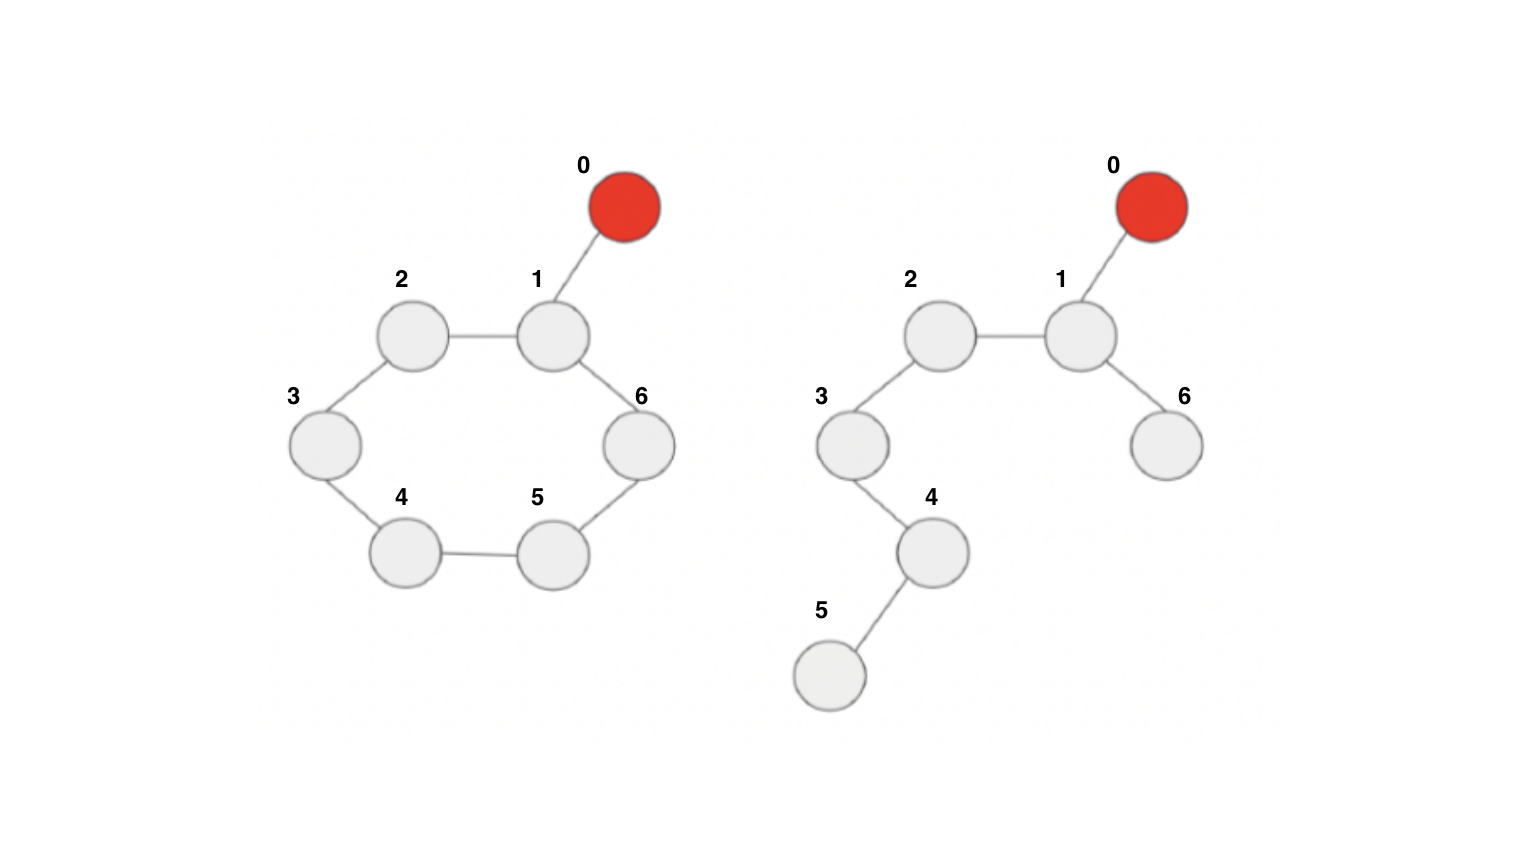
\includegraphics[scale=0.4]{/Users/dave/Desktop/projects/ee412/prj4/nodelabeling.png}    
\end{center}

The adjacency matrix is as follows.\\

A1 adjacency matrix
\[
\begin{bmatrix}
1 & 1 & 0 & 0 & 0 & 0 & 0 \\
1 & 1 & 1 & 0 & 0 & 0 & 1 \\
0 & 1 & 1 & 1 & 0 & 0 & 0 \\
0 & 0 & 1 & 1 & 1 & 0 & 0 \\
0 & 0 & 0 & 1 & 1 & 1 & 0 \\
0 & 0 & 0 & 0 & 1 & 1 & 1 \\
0 & 1 & 0 & 0 & 0 & 1 & 1
\end{bmatrix}
\]

A2 adjacency matrix
\[
\begin{bmatrix}
1 & 1 & 0 & 0 & 0 & 0 & 0 \\
1 & 1 & 1 & 0 & 0 & 0 & 1 \\
0 & 1 & 1 & 1 & 0 & 0 & 0 \\
0 & 0 & 1 & 1 & 1 & 0 & 0 \\
0 & 0 & 0 & 1 & 1 & 1 & 0 \\
0 & 0 & 0 & 0 & 1 & 1 & 0 \\
0 & 1 & 0 & 0 & 0 & 0 & 1
\end{bmatrix}
\]\\


The equation for each GNN layer is as follows.

\[
    x_{l+1} = Ax_l
\]

\(x_l^T\) for each layer is as follows. Upper one is for A1, and lower one is for A2.\\

Layer 1
\[
\begin{bmatrix}
2 & 4 & 3 & 3 & 3 & 3 & 3
\end{bmatrix}
\]
\[
\begin{bmatrix}
2 & 4 & 3 & 3 & 3 & 2 & 2
\end{bmatrix}
\]

Layer 2
\[
\begin{bmatrix}
6 & 12 & 10 & 9 & 9 & 9 & 10
\end{bmatrix}
\]
\[
\begin{bmatrix}
6 & 11 & 10 & 9 & 8 & 5 & 6
\end{bmatrix}
\]

Layer 3
\[
\begin{bmatrix}
18 & 38 & 31 & 28 & 27 & 28 & 31
\end{bmatrix}
\]
\[
\begin{bmatrix}
17 & 33 & 30 & 27 & 22 & 13 & 17
\end{bmatrix}
\]


Hence, the value of the red node becomes different at layer 3. \\



\subsection*{1-(b)}
The message function is simply identity.
\[
    M(h^k_v) = h^k_v    
\]
The aggregation function should indicate whether there exists a neighbor with the value 1.
Otherwise, the value should be 0.\\
\[
    h^{k+1}_{N(v)} = \bigcup_{u \in N(v)} M(h^k_u) = \bigcup_{u \in N(v)} h^k_u
\]
The union operation is defined as follows.
\[
    \bigcup_{u \in N(v)} h^k_u = 1 \text{ if } \exists u \in N(v) \text{ s.t. } h^k_u = 1 \text{, otherwise } 0
\]
The update rule is the union of the aggregation and itself. This indicates that the value of the node
is 1 if there exists a neighbor with the value 1, or it was initially 1. Otherwise, the value is 0.\\
\[
    h^{k+1}_v = h^{k+1}_{N(v)} \cup h^k_v
\]


\subsection*{2-(a)}

The given inequality is written in the following form.
\[
    f(\lambda x + (1-\lambda)y) > \lambda f(x) + (1-\lambda)f(y)
\]


i. GINI impurity for two class case becomes as follows.

\begin{align*}
    & f(p) = 1 - p^2 - (1-p)^2 = 2p(1-p) \\
    & f(\lambda x + (1-\lambda)y) - \lambda f(x) - (1-\lambda)f(y) \\
    &= 2(\lambda x + (1-\lambda) y) (1-\lambda x - (1-\lambda)y) - 2\lambda x (1 - x) - 2(1-\lambda)y(1 - y) \\
    &= \lambda (-\lambda x^2 + 2 \lambda x y - \lambda y^2 + x^2 - 2 x y + y^2) \\
    &= \lambda (1 - \lambda) (x - y)^2 \\
    &> 0 \text{ for } \lambda \in (0, 1) \text{ and } x \neq y
\end{align*}


ii. Entropy for two class case becomes as follows.
\begin{align*}
    & f(p) = - p\log p - (1-p)\log(1-p) \\
    & f(\lambda x + (1-\lambda)y) - \lambda f(x) - (1-\lambda)f(y) \\
    &= -(\lambda x + (1-\lambda) y) \log (\lambda x + (1-\lambda) y) + \lambda x \log x + (1-\lambda) y \log y 
\end{align*}


We apply the AM-GM Inequality to the numbers \(\lambda x\) and \((1 - \lambda)y\). This gives us
\begin{align*}
    \frac{\lambda x + (1 - \lambda)y}{2} &> \sqrt{\lambda x \cdot (1 - \lambda)y} \text{ for } \lambda \in (0, 1) \text{ and } x \neq y \\
    \log\left(\frac{\lambda x + (1 - \lambda)y}{2}\right) &> \frac{1}{2} \log(\lambda x) + \frac{1}{2} \log((1 - \lambda)y) \\
    -2\log\left(\frac{\lambda x + (1 - \lambda)y}{2}\right) &< -\log(\lambda x) - \log((1 - \lambda)y)
\end{align*}


Since \(\log(x)\) is a concave function, we can apply Jensen's Inequality to the left-hand side of the above inequality.
\begin{align*}
    -\log\left(\lambda x + (1 - \lambda)y\right) &< -2\log\left(\frac{\lambda x + (1 - \lambda)y}{2}\right) \\
    &< -\lambda \log(\lambda x) - (1 - \lambda) \log((1 - \lambda)y)
\end{align*}


iii. the accuracy measure of impurity for two class case becomes as follows.
\[
  f(p) = 1 - \max(p, 1-p)  
\]
This is not strictly concave, since it is piecewise linear. 
\begin{align*}
    f(p) &= p \text{ for } p \in [0, 1/2] \\
        &= 1 - p \text{ for } p \in [1/2, 1]
\end{align*}
For instance, \(\lambda = 1/2, x = 1/2, y = 1\) gives us 
\[
    f(\lambda x + (1-\lambda)y) - \lambda f(x) - (1-\lambda)f(y) = 0
\]




\subsection*{2-(b)}

\begin{align*}
    \text{GINI Impurity (Root node)} &= 1 - \left(\frac{5}{12}\right)^2 - \left(\frac{3}{12}\right)^2 - \left(\frac{2}{12}\right)^2 - \left(\frac{2}{12}\right)^2 \\
    \text{Accuracy (Root node)} &= 1 - \max\left(\frac{5}{12}, \frac{3}{12}, \frac{2}{12}, \frac{2}{12}\right) \\
    \text{GINI Impurity (SA or Eur node)} &= 1 - \left(\frac{5}{6}\right)^2 - \left(\frac{1}{6}\right)^2 \\
    \text{Accuracy (SA or Eur node)} &= 1 - \max\left(\frac{5}{6}, \frac{1}{6}\right) \\
    \text{GINI Impurity (Non SA or Eur node)} &= 1 - \left(\frac{2}{6}\right)^2 - \left(\frac{2}{6}\right)^2 - \left(\frac{2}{6}\right)^2 \\
    \text{Accuracy (Non SA or Eur node)} &= 1 - \max\left(\frac{2}{6}, \frac{2}{6}, \frac{2}{6}\right) \\
    \text{GINI Impurity (NA node)} &= 1 - \left(\frac{2}{4}\right)^2 - \left(\frac{2}{4}\right)^2 \\
    \text{Accuracy (NA node)} &= 1 - \max\left(\frac{2}{4}, \frac{2}{4}\right)
\end{align*}

\begin{align*}
    \text{Root node GINI impurity:} &\ 0.7083  \text{ and accuracy:} \ 0.5833 \\
    \text{SA or Eur node GINI impurity:} &\ 0.2778  \text{ and accuracy:} \ 0.1667 \\
    \text{Non SA or Eur node GINI impurity:} &\ 0.6667  \text{ and accuracy:} \ 0.6667 \\
    \text{NA node GINI impurity:} &\ 0.5  \text{ and accuracy:} \ 0.5 \\
\end{align*}



\subsection*{3-(a)}


\textbf{i.} \\


FPR is given by the following equation.

\[ p = (1 - e^{-km/n})^k \]


For \( n = 8 \times 10^9 \) and \( m = 1 \times 10^9 \) and \( k = 3, 4\), 
the false positive rate when using three hash functions is approximately 3.06\%, and when using four hash functions is approximately 2.40\%. \\


\textbf{ii.} \\


For a given array, the probability that a bit is not set by a particular member of S is \( 1 - \frac{1}{n/k} = \frac{n/k - 1}{n/k} \).
The probability that a bit remains unset by all m members is \( \left( \frac{n/k - 1}{n/k} \right)^m \).
Therefore, the probability that a bit is set (1) in a given array is \( 1 - \left( \frac{n/k - 1}{n/k} \right)^m \).
For a nonmember of S to be a false positive, it must hash to a set bit (1) in all k arrays. Hence, the overall probability of a false positive is \( \left[ 1 - \left( \frac{n/k - 1}{n/k} \right)^m \right]^k \).
The probability of a false positive when using k hash functions on a single array of n bits is \( (1 - e^{-km/n})^k \). \\



We assume the values (n = 1000 bits, m = 100 members, k = 10 hash functions):
For the former, the probability is \(0.0105\), whereas for the latter, the probability is \(0.0102\). \\


\textbf{iii.} \\

Since the FPR \( p \) for a Bloom filter:

\[ p = \left(1 - e^{-km/n}\right)^k \]

\[ \ln(p) = k \ln\left(1 - e^{-km/n}\right) \]

Differentiation with respect to \( k \) gives: 

\[ \frac{d}{dk}\ln(p) = \ln\left(1 - e^{-km/n}\right) + \frac{kme^{-km/n}}{n\left(1 - e^{-km/n}\right)} \]

We want to set this derivative to zero to find the optimal number of hash functions, \( k \):

\[ \ln\left(1 - e^{-km/n}\right) + \frac{kme^{-km/n}}{n\left(1 - e^{-km/n}\right)} = 0 \]

Suppose \(X = 1-e^{-km/n}\). Then, we have

\[
    X\ln(X) = (1-X)\ln(1-X) \implies X = 1-X \implies X = 1/2
\]

This gives us, \( 1 - e^{-km/n} = 1/2 \implies e^{-km/n} = 1/2 \implies km/n = \ln(2) \implies k = n\ln(2)/m \). \\

\subsection*{3-(b)}

\textbf{i.} \\

For \( h(x) = 2x + 1 \mod 32 \), the tail lengths are:

\begin{itemize}
    \item \( h(3) = 7 \) (\(00111\)) - Tail Length: 0
    \item \( h(1) = 3 \) (\(00011\)) - Tail Length: 0
    \item \( h(4) = 9 \) (\(01001\)) - Tail Length: 0
    \item \( h(1) = 3 \) (\(00011\)) - Tail Length: 0
    \item \( h(5) = 11 \) (\(01011\)) - Tail Length: 0
    \item \( h(9) = 19 \) (\(10011\)) - Tail Length: 0
    \item \( h(2) = 5 \) (\(00101\)) - Tail Length: 0
    \item \( h(6) = 13 \) (\(01101\)) - Tail Length: 0
    \item \( h(5) = 11 \) (\(01011\)) - Tail Length: 0
\end{itemize}

The estimated number of distinct elements is \( 2^R = 2^0 = 1 \). \\

For \( h(x) = 3x + 7 \mod 32 \), the tail lengths are:

\begin{itemize}
    \item \( h(3) = 16 \) (\(10000\)) - Tail Length: 4
    \item \( h(1) = 10 \) (\(01010\)) - Tail Length: 1
    \item \( h(4) = 19 \) (\(10011\)) - Tail Length: 0
    \item \( h(1) = 10 \) (\(01010\)) - Tail Length: 1
    \item \( h(5) = 22 \) (\(10110\)) - Tail Length: 1
    \item \( h(9) = 2 \) (\(00010\)) - Tail Length: 1
    \item \( h(2) = 13 \) (\(01101\)) - Tail Length: 0
    \item \( h(6) = 25 \) (\(11001\)) - Tail Length: 0
    \item \( h(5) = 22 \) (\(10110\)) - Tail Length: 1
\end{itemize}

The estimated number of distinct elements is \( 2^R = 2^4 = 16 \). \\

For \( h(x) = 4x \mod 32 \), the tail lengths are:

\begin{itemize}
    \item \( h(3) = 12 \) (\(01100\)) - Tail Length: 2
    \item \( h(1) = 4 \) (\(00100\)) - Tail Length: 2
    \item \( h(4) = 16 \) (\(10000\)) - Tail Length: 4
    \item \( h(1) = 4 \) (\(00100\)) - Tail Length: 2
    \item \( h(5) = 20 \) (\(10100\)) - Tail Length: 2
    \item \( h(9) = 4 \) (\(00100\)) - Tail Length: 2
    \item \( h(2) = 8 \) (\(01000\)) - Tail Length: 3
    \item \( h(6) = 24 \) (\(11000\)) - Tail Length: 3
    \item \( h(5) = 20 \) (\(10100\)) - Tail Length: 2
\end{itemize}


The estimated number of distinct elements is \( 2^R = 2^4 = 16 \). \\


\textbf{ii.} \\

As can be seen from the \( h(x) = 2x + 1 \mod 32 \), the tail lengths are all 0.
This is because the hash function always returns an odd number, and the last bit of an odd number is always 1. Hence, the tail length is always 0.
Hence, when a is even, b should not be odd. Also, a, b should not be both even, since the hash function will always return an even number and skew the results.
Therefore, a should be odd, and it is desirable to have a relative prime of \(2^k\) for a and b.\\



\end{document}